\documentclass{article}

\PassOptionsToPackage{numbers,compress}{natbib}
\usepackage[dblblindworkshop]{neurips_2026}

\usepackage{amsmath,amssymb,amsthm}
\usepackage{booktabs}
\usepackage{graphicx}
\usepackage{microtype}

\setlength{\textfloatsep}{7pt plus 1pt minus 2pt}
\setlength{\floatsep}{7pt plus 1pt minus 2pt}
\setlength{\intextsep}{7pt plus 1pt minus 2pt}
\setlength{\abovedisplayskip}{4pt plus 1pt minus 1pt}
\setlength{\belowdisplayskip}{4pt plus 1pt minus 1pt}
\setlength{\abovedisplayshortskip}{2pt plus 1pt minus 1pt}
\setlength{\belowdisplayshortskip}{2pt plus 1pt minus 1pt}

\newtheorem{proposition}{Proposition}
\newtheorem{theorem}{Theorem}
\newtheorem{corollary}{Corollary}

\newcommand{\test}{\textsc{Test}}
\newcommand{\trust}{\textsc{Trust}}
\newcommand{\dropa}{\textsc{Drop}}
\newcommand{\risk}{\mathcal{R}}

\title{RiskTriage: Calibrating When Physical Validation Is Needed
in Computational Catalyst Discovery}

\author{Anonymous Authors}

\begin{document}

\maketitle

\begin{abstract}
Materials-AI models can rank thousands of candidates, but deployment still requires deciding which predictions are reliable enough to act on without another physical experiment.
We treat this simulation-to-experiment step as a three-action decision (\trust, \test, or \dropa) and calibrate uncertainty to downstream experimental risk $\risk$, the expected rate of wrong \trust/\dropa\ actions, rather than to predictive coverage alone.
On 179 OCx24 HER catalysts and 20 grouped splits, the minimum testing fraction $T(r)=\min_{\pi:\,\risk(\pi)\le r}\Pr(\test)$ at $\risk\le 0.10$ is $8.4\%$ [4.2, 13.4] for RAC/CRC versus $16.5\%$ [9.2, 24.4] for uncertainty sampling and $25.9\%$ [22.3, 29.6] for split conformal prediction (bootstrap 95\% CIs; the RAC/CRC and uncertainty intervals overlap at this $r$).
A cost-aware Bayes rule empties the testing region at the predicted cap $c_E\ge 1/2$, while max-min interval RAC stays at $7.4\%$ past that cap.
At the default CRC target $r^\star=0.15$ (not the same as $T(0.10)$), unseen alloy families trigger $2.9\times$ more validation ($7.4\%\to 21.2\%$).
RiskTriage is a post-hoc layer on a frozen predictor: it does not add DFT calls, GNN parameters, or extra sequence length.
\end{abstract}

\section{Introduction}

AI-accelerated materials screening can evaluate far more candidates than can be synthesized and tested
\citep{butler2018ml,jain2013materials,ramprasad2017materials,lookman2019active,merchant2023scaling}.
Deployment still requires a decision that property prediction does not answer: when is computational evidence reliable enough to skip another physical experiment?
\citep{chow1970reject,geifman2017selective,angelopoulos2021gentle}.
That question sits between AI-guided design and experimental workflow integration
\citep{kusne2020closedloop,szymanski2023autonomous,floresleonar2020maps}.
A ranker can be accurate and still operationally poor if its uncertainty sends nearly every ambiguous candidate to the laboratory, or if it saves experiments by accepting unreliable extrapolations
\citep{tran2021active,gruich2023trust,tibshirani2019covariate}.

The distinction is sharp in catalysis, where idealized computational structures, realized phases, and measured electrochemical behavior need not coincide
\citep{chanussot2021oc20,tran2023oc22,abed2024ocx,bozalginesta2025heterogeneous}.
OCx24 was built to narrow this simulation-to-experiment gap: 572 synthesized samples, 441 gas-diffusion electrodes, and computational screening over roughly 20{,}000 inorganic materials
\citep{abed2024ocx}.
Its HER task is a useful translational regime: computational descriptors explain substantial experimental variation, but residual error is large enough that physical validation still matters
\citep{abed2024ocx,gruich2023trust}.

A wide conformal interval may be statistically valid, yet if every interval that crosses a performance threshold triggers an experiment, high coverage becomes an impractically high testing rate
\citep{shafer2008tutorial,angelopoulos2024crc}.
Uncertainty sampling spends experiments on high-variance candidates even when resolving that variance would not change the action
\citep{lookman2019active,tran2021active}.
Conformal Risk Control (CRC)~\citep{angelopoulos2024crc} and Risk-Averse Calibration (RAC)~\citep{kiyani2025rac} instead calibrate uncertainty to the decision maker's downstream loss.

We add a decision layer, RiskTriage, between computational screening and physical characterization.
Given a calibrated probability that a catalyst exceeds a practical threshold, it chooses among \trust, \test, and \dropa.
We study a \emph{risk-budget} regime, minimizing physical testing subject to $\risk\le r$, and a \emph{cost-aware} regime, where Bayes decision theory trades experimental cost against false acceptance and false rejection
\citep{chow1970reject,angelopoulos2024crc,kiyani2025rac}.

\begin{figure}[t]
\centering
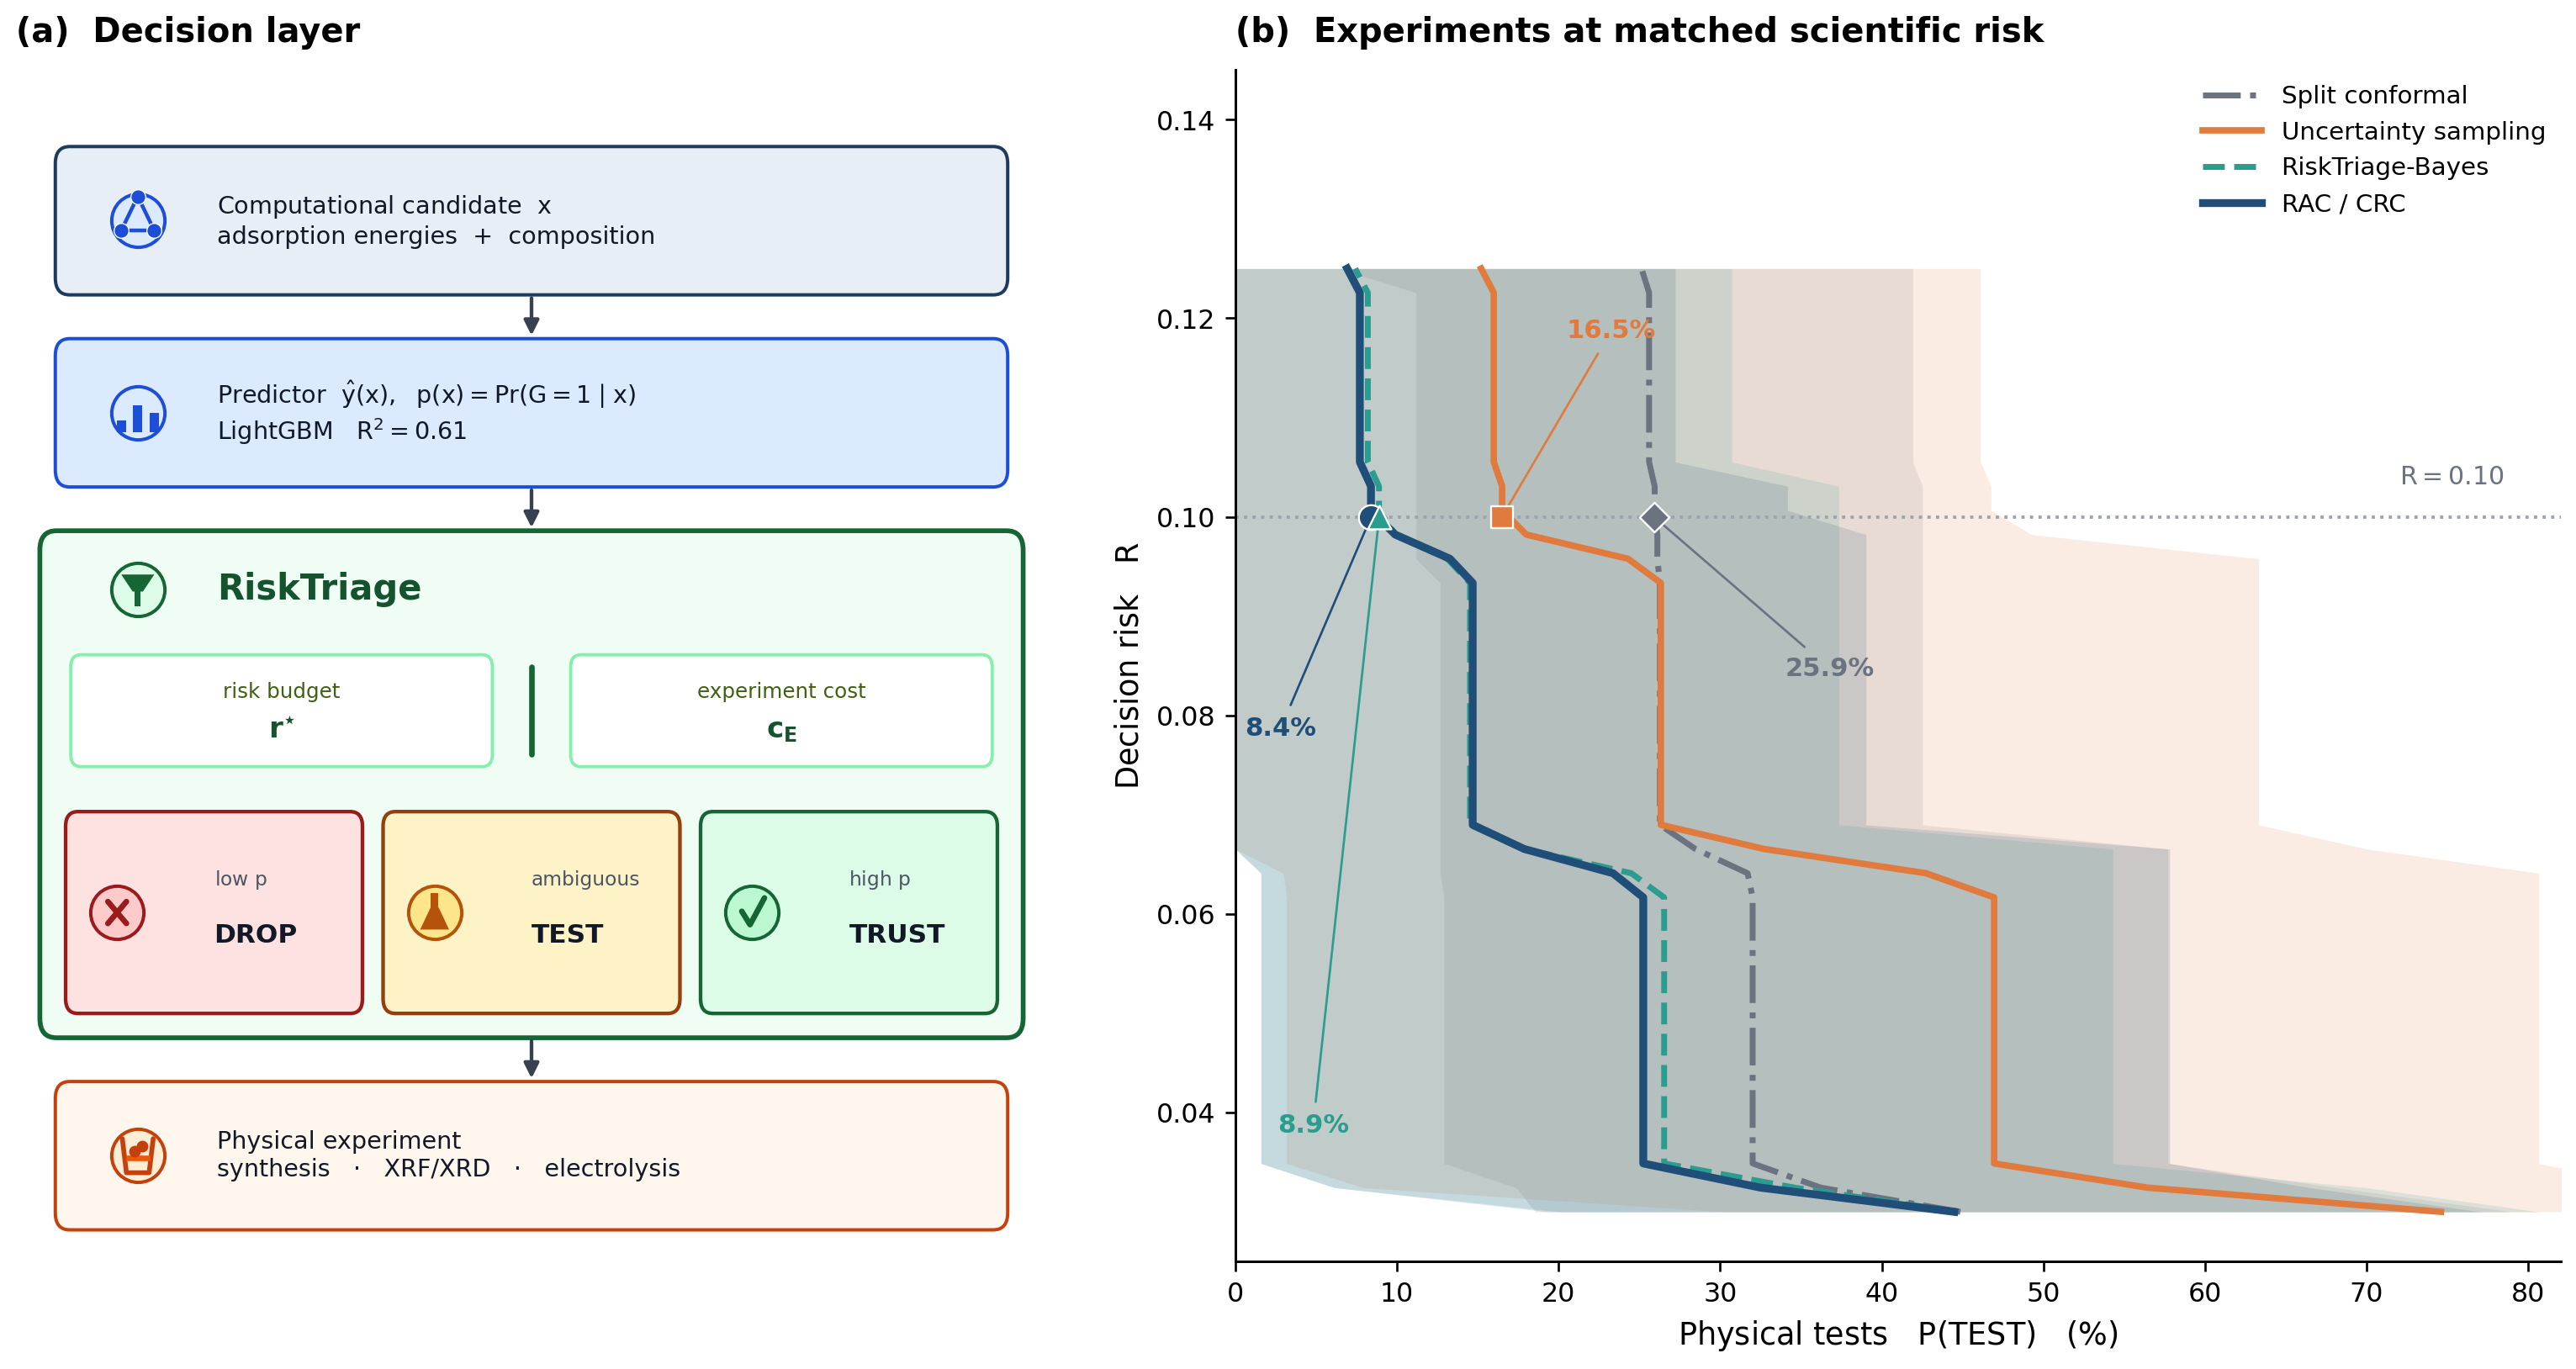
\includegraphics[width=\linewidth]{figures/fig1_risktriage.png}
\caption{\textbf{RiskTriage as a lab decision layer.}
\textbf{(a)}~A predictor estimates $p(x)=\Pr(G{=}1\mid x)$; RiskTriage chooses \dropa/\test/\trust\ from a risk budget or experiment cost $c_E$.
\textbf{(b)}~Physical-testing fraction versus decision risk (mean and 2.5--97.5\% band over 20 grouped splits). Markers are matched-risk $T(0.10)$: RAC/CRC $8.4\%$, RiskTriage-Bayes $8.9\%$, uncertainty sampling $16.5\%$, split conformal $25.9\%$. Lower-left is better.}
\label{fig:risktriage}
\end{figure}

\section{Methodology}

\textbf{Data and prediction task.}
We use the OCx24 HER experimental targets after composition aggregation and cleaning~\citep{abed2024ocx}.
The task has $N=179$ samples, 166 sample-ID groups, and 45 alloy families.
The target is experimental $V_{50}$ versus SHE (less negative is better).
Success is the training-split empirical top quartile, $G_i=\mathbf{1}\{Y_i\ge y^\star\}$, with global 75th percentile $y^\star=-1.266~\mathrm{V}$ (25.1\% positives); $y^\star$ is frozen from the training partition in each split.

Features are the OCx24 adsorption-energy descriptors plus composition descriptors~\citep{abed2024ocx,ward2018matminer}.
We compare linear regression, ridge, random forests, and LightGBM~\citep{hoerl1970ridge,breiman2001rf,ke2017lightgbm}.
Evaluation is group-aware (replicate sample IDs do not cross splits) and averaged over 20 grouped splits.
RiskTriage is applied post hoc to a frozen LightGBM ensemble: no extra DFT, no extra GNN, no longer token sequence.

\textbf{Three-action experimental decision.}
For candidate $x$, let $p(x)=\Pr(G=1\mid X=x)$.
Actions are $a(x)\in\{\trust,\test,\dropa\}$, with false-trust cost $c_{\mathrm{FP}}$, false-drop cost $c_{\mathrm{FN}}$, and test cost $c_E$:
$R_{\trust}(p)=(1-p)c_{\mathrm{FP}}$,
$R_{\dropa}(p)=pc_{\mathrm{FN}}$,
$R_{\test}(p)=c_E$.

\begin{proposition}[Bayes-optimal physical-testing region]
\label{prop:bayes}
If $c_E\le c_{\mathrm{FP}}c_{\mathrm{FN}}/(c_{\mathrm{FP}}+c_{\mathrm{FN}})$,
the Bayes-optimal policy is
\[
a^\star(p)=
\begin{cases}
\dropa, & p\le c_E/c_{\mathrm{FN}},\\
\test, & c_E/c_{\mathrm{FN}} < p < 1-c_E/c_{\mathrm{FP}},\\
\trust, & p\ge 1-c_E/c_{\mathrm{FP}}.
\end{cases}
\]
When the inequality on $c_E$ fails, the \test\ region is empty.
\end{proposition}

Experimentation is then optimal only when uncertainty is decision-relevant.
For $c_{\mathrm{FP}}=c_{\mathrm{FN}}=1$, testing disappears once $c_E\ge 1/2$.
Proofs are in Appendix~\ref{app:proofs}.

\textbf{Risk-budget calibration.}
Bayes answers whether one experiment is worth $c_E$.
The complementary quantity is the minimum testing fraction at a scientific risk budget $r$,
\[
T(r)=\min_{\pi:\,\risk(\pi)\le r}\Pr_\pi(\test),
\qquad
\risk=\mathbb{E}[L_{\mathrm{triage}}],
\]
with
$L_{\mathrm{triage}}=\mathbf{1}\{a=\trust,G=0\}+\mathbf{1}\{a=\dropa,G=1\}$.
CRC/RAC chooses a nested-set threshold to control $\risk$ while minimizing deferral to \test.
For this three-action utility the robust RAC and CRC actions coincide, so we report them jointly as RAC/CRC.
$T(r)$ is read off the realized (test rate, risk) frontier of each method; it is \emph{not} the same as running CRC with target $r^\star=r$
(Appendix~\ref{app:frontiers}).
At target $r^\star=0.10$, CRC tests $14.3\%$ with realized risk $0.093$; Table~\ref{tab:main}b reports the tighter matched-risk reading $T(0.10)=8.4\%$.

Baselines: point prediction, uncertainty sampling by ensemble standard deviation, split conformal prediction, and probability thresholds.
Split conformal tests a candidate whenever its interval straddles $y^\star$.
Split construction, \(\hat p\), and conformal scores are specified in Appendix~\ref{app:details}.

\begin{theorem}[Safe threshold action]
\label{thm:cp}
If $C_\alpha(X)=[L_\alpha(X),U_\alpha(X)]$ satisfies
$\Pr\{Y\in C_\alpha(X)\}\ge1-\alpha$, and we \trust\ when $L_\alpha(X)\ge y^\star$, \dropa\ when $U_\alpha(X)<y^\star$, and otherwise \test, then $\Pr(\text{wrong \trust\ or \dropa})\le\alpha$.
\end{theorem}
Theorem~\ref{thm:cp} gives safety of split conformal prediction, not experimental efficiency.

\begin{table}[t]
\centering
\caption{\textbf{Prediction fidelity and experimental efficiency.}
(a)~Grouped HER prediction, 20 splits. Bold: best in column (ties at displayed precision).
(b)~Minimum testing fraction $T(r)$ (\%) at matched maximum decision risk. Bold: lowest mean $T(r)$ in the row, not a highlighted operating point.
RiskTriage-Bayes is the matched-risk reading of the cost-aware Bayes policy, not the default $c_E=0.2$ point (which tests $2.0\%$; Appendix~\ref{app:robustness}a).
Brackets: bootstrap 95\% CIs.
The $r=0.03$ row uses 19 splits for RAC/CRC, Bayes, and split CP (one split never reached $\risk\le 0.03$).}
\label{tab:main}
\scriptsize
\renewcommand{\arraystretch}{0.92}
\setlength{\tabcolsep}{3pt}
\begin{tabular}{lcccc}
\toprule
\multicolumn{5}{c}{\textbf{(a) Base prediction performance}}\\
\midrule
Model & $R^2$ & MAE & RMSE & Spearman\\
\midrule
Linear & 0.518 & 0.088 & 0.112 & 0.718\\
Ridge & 0.562 & 0.083 & 0.106 & 0.751\\
Random forest & 0.602 & \textbf{0.079} & \textbf{0.101} & 0.783\\
LightGBM & \textbf{0.605} & \textbf{0.079} & \textbf{0.101} & \textbf{0.791}\\
\midrule
\multicolumn{5}{c}{\textbf{(b) Physical testing required at matched decision risk}}\\
\midrule
Max risk $r$ & RAC/CRC & RiskTriage-Bayes & Uncertainty & Split CP\\
\midrule
0.03 &
\textbf{44.5 [36.9, 53.1]} &
44.7 [36.7, 53.9] &
74.6 [65.2, 82.5] &
44.9 [37.0, 53.2]\\
0.05 &
\textbf{25.2 [18.3, 32.6]} &
26.5 [19.3, 33.9] &
47.0 [35.3, 58.0] &
32.0 [26.8, 37.4]\\
0.075 &
14.7 [9.3, 20.5] &
\textbf{14.5 [9.2, 20.1]} &
26.3 [16.4, 36.5] &
26.3 [22.7, 29.8]\\
0.10 &
\textbf{8.4 [4.2, 13.4]} &
8.9 [4.3, 14.3] &
16.5 [9.2, 24.4] &
25.9 [22.3, 29.6]\\
0.125 &
\textbf{6.9 [3.3, 11.2]} &
7.4 [3.4, 12.2] &
15.2 [8.1, 22.9] &
25.1 [21.1, 28.9]\\
\bottomrule
\end{tabular}
\end{table}

\section{Results and Discussion}

\textbf{Matched-risk testing.}
Table~\ref{tab:main}a checks that the base predictor reproduces the known OCx24 HER signal before we measure experimental efficiency.
LightGBM attains $R^2=0.605$, MAE $=0.079$~V, RMSE $=0.101$~V, and Spearman $0.791$, matching the ${\sim}0.59$--$0.61$ simulation-to-experiment HER $R^2$ reported for OCx24.
At three-decimal MAE, random forest is tied (unrounded: $0.0786$ vs.\ $0.0793$).
Screening is informative and still imperfect, so triage is relevant.

Figure~\ref{fig:risktriage} and Table~\ref{tab:main}b report the primary endpoint $T(r)$.
At $\risk\le 0.10$, RAC/CRC tests $8.4\%$ [4.2, 13.4] of candidates, RiskTriage-Bayes $8.9\%$ [4.3, 14.3], uncertainty sampling $16.5\%$ [9.2, 24.4], and split conformal $25.9\%$ [22.3, 29.6].
The RAC/CRC and uncertainty intervals overlap at this $r$; the comparison is cleaner at $r=0.05$ ($25.2$ [18.3, 32.6] vs.\ $47.0$ [35.3, 58.0]).
Point prediction tests $0\%$ and incurs risk $0.140$ (Appendix~\ref{app:frontiers}a).
The reverse frontier agrees: at a 10\% testing budget, RAC/CRC risk is $0.096$ [0.074, 0.122] versus $0.113$ [0.086, 0.142] for uncertainty sampling; at 30\% testing the risks are $0.043$ and $0.078$ (Appendix~\ref{app:frontiers}c).
Split conformal reaches a testing fraction below 10\% on only 2 of 20 seeds, so that reverse cell is omitted.

Split conformal at $\alpha=0.1$ covers $Y$ at rate $94.2\%$ and almost eliminates wrong non-test actions, but tests $75.0\%$ of candidates at that default operating point---not at $T(0.10)$.
It is statistically safe and experimentally conservative.

\textbf{Cost.}
With $c_{\mathrm{FP}}=c_{\mathrm{FN}}=1$, Proposition~\ref{prop:bayes} gives the testing region $c_E<p(x)<1-c_E$, which empties at $c_E=1/2$.
Across 20 seeds, Bayes testing falls from $5.9\%$ at $c_E=0.01$ to $0.8\%$ at $c_E=0.40$ and to $0\%$ for $c_E\ge 0.60$ (Appendix~\ref{app:robustness}a).
Max-min interval RAC stays at $7.4\%$ for every $c_E\in[0.01,0.80]$, including above the Bayes cap.
Risk calibration and cost-aware action selection are different knobs.

\textbf{Unfamiliar chemistry.}
These OOD numbers use the default CRC target $r^\star=0.15$ (mean test rate $7.4\%$, risk $0.114$), not matched-risk $T(0.10)$.
Holding out alloy families raises RAC/CRC testing from $7.4\%$ to $21.2\%$ ($2.9\times$; $0.212/0.074\approx 2.86$) while risk moves from $0.114$ to $0.092$ (Appendix~\ref{app:robustness}b).
Split conformal tests $75.0\%$ IID and $81.1\%$ OOD.

\textbf{Discovery utility.}
RiskTriage is not a ranking method.
Retrospective replay gives AUDC $0.929$ versus $0.927$ for LightGBM rank (paired $\Delta=+0.002$, 95\% CI $[0.000,0.006]$, $\Pr(\Delta>0)=0.63$; Appendix~\ref{app:discovery}).
The gain is calibrated abstention, not discovery.

Intermediate XRF/XRD, used to update $p(x)$, lowers later electrochemical testing from $7.4\%$ to $5.1\%$ (risk $0.114\to 0.125$).
Hard-dropping unmatched samples cuts testing to $1.1\%$ but raises risk to $0.146$ and discards $2.1\%$ good catalysts (Appendix~\ref{app:robustness}c).

\textbf{Limitations.}
$n=179$; CIs on $T(0.10)$ are wide and overlap the uncertainty-sampling interval.
The study is retrospective, not a closed-loop laboratory deployment.
The top-quartile threshold is an evaluation device, not an application-specific spec.
OCx24 does not expose a logging policy over the ${\sim}20$k computational candidates; conclusions concern the observed experimental population (Appendix~\ref{app:ipw}).

\section{Conclusion}

RiskTriage asks when computational evidence is reliable enough to skip another physical experiment.
On OCx24 HER, calibrating uncertainty to decision risk reduces physical validation at a fixed scientific-error tolerance, leaves ranking essentially unchanged, shuts off testing when experiments are too costly, and requests more validation on unseen alloy families.
The operational principle is that uncertainty should be calibrated to the physical decision it controls.

\bibliographystyle{unsrtnat}
\bibliography{references}

\newpage
\appendix

\section{Theory and Proofs}
\label{app:proofs}

\textbf{Proof of Proposition~\ref{prop:bayes}.}
Conditional risks are
$R_{\trust}(p)=(1-p)c_{\mathrm{FP}}$,
$R_{\dropa}(p)=pc_{\mathrm{FN}}$,
$R_{\test}(p)=c_E$.
\test\ is no worse than \dropa\ iff $p\ge c_E/c_{\mathrm{FN}}$, and no worse than \trust\ iff $p\le 1-c_E/c_{\mathrm{FP}}$.
The interval is nonempty iff
$c_E\le c_{\mathrm{FP}}c_{\mathrm{FN}}/(c_{\mathrm{FP}}+c_{\mathrm{FN}})$.
\hfill$\square$

\begin{corollary}[Monotonicity in experimental cost]
For fixed $p(x)$, the physical-testing fraction is non-increasing in $c_E$.
\end{corollary}

\begin{proof}
The Bayes \test\ set
$\mathcal{T}(c)=\{x: c/c_{\mathrm{FN}} < p(x) < 1-c/c_{\mathrm{FP}}\}$
shrinks as $c$ increases, so $\Pr(X\in\mathcal{T}(c))$ is non-increasing.
\end{proof}

\textbf{Proof of Theorem~\ref{thm:cp}.}
Let
$E=\{a(X)=\trust,\,Y<y^\star\}\cup\{a(X)=\dropa,\,Y\ge y^\star\}$.
Wrong \trust\ implies $Y\notin C_\alpha(X)$; wrong \dropa\ likewise.
Thus $E\subseteq\{Y\notin C_\alpha(X)\}$ and $\Pr(E)\le\alpha$.
\hfill$\square$

\textbf{Uncertainty sampling is not decision-optimal.}
Let $y^\star=0$ and unit false-decision costs.
A law on $\{-100,-1\}$ can have large variance and $\mathrm{VOI}=0$; a balanced $\{\pm 1\}$ law has smaller variance and $\mathrm{VOI}=1/2$.

\section{Experimental Details}
\label{app:details}

The HER table has 179 aggregated samples, 166 sample-ID groups, 45 alloy families, and 43 XRD-matched samples.
Unless stated, $c_{\mathrm{FP}}=c_{\mathrm{FN}}=1$, $c_E=0.2$, $r^\star=0.15$, and conformal miscoverage $\alpha=0.10$.
The principal predictor is LightGBM; linear/ridge/RF check that efficiency conclusions are not an artifact of a weak base model.
Default CRC/RAC numbers (test rate $7.4\%$, risk $0.114$) are this $r^\star=0.15$ operating point.
Matched-risk $T(r)$ traces the dense frontier of each method and takes the minimum test rate with realized $\risk\le r$.

\textbf{Splits.}
Each of the 20 seeds partitions the 166 sample-ID groups in proportions $0.65/0.175/0.175$ train/calibration/test (remainder to test), then maps groups to rows.
No sample ID appears in more than one role.
The success threshold $y^\star$ is the 75th percentile of \emph{training} $Y$ in that split.
Leave-one-family-out $R^2$ in Table~\ref{tab:main}a uses composition-family folds, not these 65/17.5/17.5 splits.
OOD splits $k$-means ($k=8$) group-feature centroids, hold out two clusters as test, and split the remaining groups $75/25$ train/calibration.

\textbf{Predictor, $\hat p$, and variance.}
Decision policies use a five-member LightGBM ensemble fit on train only (member seeds offset; median imputation and standardization in-pipeline).
The point prediction $\hat y(x)$ is the member mean; the ensemble scale $\hat\sigma_{\mathrm{ens}}(x)$ is the member standard deviation, floored at $10^{-4}$.
A training residual MAD $\tau$ is added in quadrature,
$\sigma(x)=\sqrt{\hat\sigma_{\mathrm{ens}}(x)^2+\tau^2}$.
We do not apply a second-stage probability calibrator (no Platt/isotonic step).
The cost-aware rule uses the Gaussian tail
$\hat p(x)=\Pr\bigl(N(\hat y(x),\sigma(x)^2)\ge y^\star\bigr)$.
Uncertainty sampling ranks candidates by $\hat\sigma_{\mathrm{ens}}$ (not $\sigma$), tests the top fraction, and point-classifies the rest ($\trust$ iff $\hat y\ge y^\star$).

\textbf{Split conformal and RAC/CRC.}
The nonconformity score on calibration is the normalized residual
$s_i=|Y_i-\hat y(x_i)|/\sigma(x_i)$.
The split-conformal threshold is the empirical quantile at
$\lceil(n_{\mathrm{cal}}+1)(1-\alpha)\rceil/n_{\mathrm{cal}}$ (``higher'' quantile), $\alpha=0.10$.
Prediction sets are nested intervals $[\hat y\pm\lambda\sigma]$.
A candidate is tested iff the interval straddles $y^\star$.
RAC/CRC takes the smallest $\lambda$ on a geometric grid such that the finite-sample CRC bound
$(n/(n+1))\widehat R_n(\lambda)+B/(n+1)$ on triage risk is at most $r^\star$, with $B=\max(c_{\mathrm{FP}},c_{\mathrm{FN}})$.

\section{Calibration and Risk--Testing Frontiers}
\label{app:frontiers}

Table~\ref{tab:app_frontiers}a is the default operating point ($r^\star=0.15$ for CRC/RAC, $\alpha=0.10$ for split CP).
Table~\ref{tab:app_frontiers}b is CRC/RAC when the \emph{target} $r^\star$ varies; this is not $T(r)$.
At target $r^\star=0.10$, CRC tests $14.3\%$ with realized risk $0.093$; $T(0.10)=8.4\%$ in Table~\ref{tab:main}b is the tighter matched-risk reading of the same frontier family.
Table~\ref{tab:app_frontiers}c is the reverse frontier $R(t)$.
CRC/RAC false-\trust\ and false-\dropa\ rates at the default point are $0.176$ and $0.101$ (20-seed means from the same runs as (a)); split conformal yields $0$ and $0.012$.

\begin{table}[h]
\centering
\caption{\textbf{Calibration and frontiers} (20 grouped splits).
(a)~Default operating points.
(b)~CRC/RAC at target $r^\star$ (not $T(r)$).
(c)~Minimum decision risk at a fixed testing budget $t$.
Bold in (c): RAC/CRC cells used in the main text.}
\label{tab:app_frontiers}
\small
\begin{tabular}{lcccccc}
\toprule
\multicolumn{7}{c}{\textbf{(a) Default calibration}}\\
\midrule
Method & $P(\test)$ & Wrong non-test & $\risk$ & Full risk & Coverage & Width\\
\midrule
Point predictor & 0.000 & 0.140 & 0.140 & 0.140 & -- & --\\
Uncalibrated Bayes & 0.020 & 0.125 & 0.125 & 0.129 & 0.14 & 0.04\\
CRC/RAC ($r^\star=0.15$) & 0.074 & 0.114 & 0.114 & 0.129 & 0.14 & 0.04\\
Split CP ($\alpha=0.10$) & 0.750 & 0.003 & 0.003 & 0.153 & 0.942 & 0.60\\
\midrule
\multicolumn{7}{c}{\textbf{(b) CRC/RAC at target $r^\star$}}\\
\midrule
$r^\star$ & 0.05 & 0.10 & 0.15 & 0.20 & 0.30 & 0.40\\
Test fraction & 0.493 & 0.143 & 0.074 & 0.025 & 0.008 & 0.000\\
Realized $\risk$ & 0.028 & 0.093 & 0.114 & 0.130 & 0.139 & 0.140\\
\midrule
\multicolumn{7}{c}{\textbf{(c) Reverse frontier $R(t)$}}\\
\midrule
Budget $t$ & 5\% & 10\% & 20\% & 30\% & 50\% & \\
RAC/CRC & 0.127 [0.098, 0.158] & \textbf{0.096 [0.074, 0.122]} &
0.064 [0.047, 0.084] & 0.043 [0.028, 0.058] & 0.017 [0.008, 0.027] & \\
Uncertainty & 0.140 [0.112, 0.171] & 0.113 [0.086, 0.142] &
0.088 [0.067, 0.109] & 0.078 [0.060, 0.096] & 0.055 [0.042, 0.068] & \\
\bottomrule
\end{tabular}
\end{table}

\section{Deployment Robustness}
\label{app:robustness}

\begin{table}[h]
\centering
\caption{\textbf{Deployment robustness.}
(a)~Mean $P(\test)$ (\%) vs.\ $c_E$. Bold: empty testing region after the Bayes cap $c_E^\star=1/2$.
(b)~IID vs.\ held-out-family chemistry at $r^\star=0.15$ (not $T(0.10)$).
(c)~XRF/XRD before electrolysis, same default CRC point.}
\label{tab:app_robustness}
\small
\begin{tabular}{lcccc}
\toprule
\multicolumn{5}{c}{\textbf{(a) Experimental-cost sensitivity}}\\
\midrule
$c_E$ & Bayes & Calibrated + cost & Interval RAC & Interval + cap\\
\midrule
0.01  & 5.9 & 7.5 & 7.4 & 7.4\\
0.025 & 4.4 & 7.4 & 7.4 & 7.4\\
0.05  & 3.8 & 7.0 & 7.4 & 7.4\\
0.10  & 3.0 & 7.5 & 7.4 & 7.4\\
0.20  & 2.0 & 7.4 & 7.4 & 7.4\\
0.40  & 0.8 & 7.4 & 7.4 & 7.4\\
0.60  & \textbf{0} & \textbf{0} & 7.4 & \textbf{0}\\
0.80  & \textbf{0} & \textbf{0} & 7.4 & \textbf{0}\\
\midrule
\multicolumn{5}{c}{\textbf{(b) Composition-OOD at $r^\star=0.15$}}\\
\midrule
Method & IID test & OOD test & IID $\risk$ & OOD $\risk$\\
\midrule
CRC/RAC & 0.074 & 0.212 & 0.114 & 0.092\\
Split CP & 0.750 & 0.811 & 0.003 & 0.006\\
\midrule
\multicolumn{5}{c}{\textbf{(c) Intermediate characterization}}\\
\midrule
Policy & $P(\test)$ & $\risk$ & Tests avoided & Good lost\\
\midrule
Direct ($X$ only) & 0.074 & 0.114 & -- & --\\
Re-predict with XRF/XRD & 0.051 & 0.125 & -- & --\\
Drop unmatched & 0.011 & 0.146 & 0.039 & 0.021\\
\bottomrule
\end{tabular}
\end{table}

Interval RAC continues to prefer \test\ on straddling sets for all $c_E<1$, which is why it stays at $7.4\%$ after $c_E=1/2$.

\section{Retrospective Discovery Utility}
\label{app:discovery}

\begin{table}[h]
\centering
\caption{\textbf{Retrospective experimental-budget replay.}
AUDC: area under the discovery curve.
Last column: mean experiments to 80\% recall of the experimental top decile (blank when 80\% is never reached).
Bold: best AUDC. The $B=5$ recall figures in the text ($0.617$ vs.\ $0.604$) are 20-seed means from the same replay, not a separate experiment.}
\label{tab:app_discovery}
\small
\begin{tabular}{lcc}
\toprule
Policy & AUDC & Experiments to 80\% recall\\
\midrule
RiskTriage & \textbf{0.929} & 10.3\\
ML rank & 0.927 & 10.3\\
UCB & 0.925 & 10.5\\
Expected improvement & 0.918 & 10.8\\
VOI & 0.797 & 16.6\\
Random & 0.546 & 26.2\\
Variance / conformal width & 0.541 & 26.1\\
Sabatier ($|E_{\mathrm{H}}|$) & 0.266 & ${\sim}30$\\
\bottomrule
\end{tabular}
\end{table}

Paired bootstrap $\Delta\mathrm{AUDC}=+0.002$ $[0.000,0.006]$, $\Pr(\Delta>0)=0.63$.
At budget $B=5$, RiskTriage recall of the top decile is $0.617$ versus $0.604$ for ML rank (mean best-catalyst regret $0.005$ vs.\ $0.017$).
By $B=10$ both reach $0.971$ recall.

\section{Selection-Bias Sensitivity}
\label{app:ipw}

XRD match is treated as a binary proxy for electrochemical selection.
A logistic regression on the computational features $X$ (standardized; default $\ell_2$) estimates $\hat\pi(x)=\Pr(\mathrm{matched}\mid X)$.
Probabilities are clipped to $[0.05,0.95]$; unmatched rows receive weight $0$.
Matched rows receive $w(x)=1/\hat\pi(x)$, then renormalized to mean $1$ on the matched subset (no further stabilization).
A ridge regressor is fit on the 43 matched samples with these weights; MAE $0.044$ (vs.\ $0.045$ unweighted) is computed on that same matched subset, so it is an in-sample sensitivity check, not a held-out IPW estimate.
XRD match is not the historical logging policy, so this does not identify off-policy performance.

\end{document}
